\documentclass[11pt]{report}

\newcommand{\coursetitle}{Machine Learning}
% ============================================================
%  Shared preamble for all course notes
%  Loaded from each course's main.tex via % ============================================================
%  Shared preamble for all course notes
%  Loaded from each course's main.tex via % ============================================================
%  Shared preamble for all course notes
%  Loaded from each course's main.tex via \input{../common/preamble}
% ============================================================

% ---------- Page layout & fonts ----------
\usepackage[utf8]{inputenc}
\usepackage[T1]{fontenc}
\usepackage{lmodern}
\usepackage{microtype}
\usepackage[a4paper, margin=2.5cm]{geometry}
\usepackage{parskip}               % space between paragraphs, no indent
\usepackage{fancyhdr}

% ---------- Math ----------
\usepackage{amsmath, amssymb, amsthm}
\usepackage{mathtools}
\usepackage{bm}

% ---------- Figures, tables, plots ----------
\usepackage{graphicx}
\usepackage{float}
\usepackage{caption}
\usepackage{subcaption}
\usepackage{booktabs}
\usepackage{tikz}
\usetikzlibrary{arrows.meta, positioning, shapes, calc, fit}
\usepackage{pgfplots}
\pgfplotsset{compat=1.17}
\graphicspath{{figures/}}

% ---------- Lists, code, colored boxes ----------
\usepackage{enumitem}
\usepackage{xcolor}
\usepackage{listings}
\usepackage[most]{tcolorbox}

% ---------- References ----------
\usepackage[numbers]{natbib}
\usepackage[colorlinks=true, linkcolor=blue!60!black,
            citecolor=green!50!black, urlcolor=blue!70!black]{hyperref}
\usepackage[capitalise, noabbrev]{cleveref}   % must come after hyperref

% ---------- Header / footer ----------
\pagestyle{fancy}
\fancyhf{}
\fancyhead[L]{\nouppercase{\leftmark}}
\fancyhead[R]{\coursetitle}
\fancyfoot[C]{\thepage}
\setlength{\headheight}{14.5pt}

% ---------- Theorem-like environments ----------
\theoremstyle{definition}
\newtheorem{definition}{Definition}[chapter]
\newtheorem{example}{Example}[chapter]
\newtheorem{exercise}{Exercise}[chapter]

\theoremstyle{plain}
\newtheorem{theorem}{Theorem}[chapter]
\newtheorem{lemma}[theorem]{Lemma}
\newtheorem{proposition}[theorem]{Proposition}
\newtheorem{corollary}[theorem]{Corollary}

\theoremstyle{remark}
\newtheorem*{remark}{Remark}
\newtheorem*{note}{Note}

% ---------- Highlight boxes ----------
% \begin{keyidea} ... \end{keyidea}   -- main takeaway of a lecture
% \begin{intuition} ... \end{intuition}
\newtcolorbox{keyidea}[1][Key Idea]{
  colback=blue!4, colframe=blue!50!black, fonttitle=\bfseries,
  title=#1, breakable}
\newtcolorbox{intuition}[1][Intuition]{
  colback=green!4, colframe=green!40!black, fonttitle=\bfseries,
  title=#1, breakable}
\newtcolorbox{warning}[1][Caution]{
  colback=red!4, colframe=red!50!black, fonttitle=\bfseries,
  title=#1, breakable}

% ---------- Code listings (Python by default) ----------
\lstdefinestyle{notes}{
  language=Python,
  basicstyle=\ttfamily\small,
  keywordstyle=\color{blue!70!black}\bfseries,
  commentstyle=\color{green!45!black}\itshape,
  stringstyle=\color{red!60!black},
  numbers=left, numberstyle=\tiny\color{gray},
  frame=single, rulecolor=\color{gray!40},
  backgroundcolor=\color{gray!5},
  breaklines=true, showstringspaces=false, tabsize=4,
  captionpos=b
}
\lstset{style=notes}

% ---------- Shared math notation ----------
\input{../common/macros}

% ============================================================

% ---------- Page layout & fonts ----------
\usepackage[utf8]{inputenc}
\usepackage[T1]{fontenc}
\usepackage{lmodern}
\usepackage{microtype}
\usepackage[a4paper, margin=2.5cm]{geometry}
\usepackage{parskip}               % space between paragraphs, no indent
\usepackage{fancyhdr}

% ---------- Math ----------
\usepackage{amsmath, amssymb, amsthm}
\usepackage{mathtools}
\usepackage{bm}

% ---------- Figures, tables, plots ----------
\usepackage{graphicx}
\usepackage{float}
\usepackage{caption}
\usepackage{subcaption}
\usepackage{booktabs}
\usepackage{tikz}
\usetikzlibrary{arrows.meta, positioning, shapes, calc, fit}
\usepackage{pgfplots}
\pgfplotsset{compat=1.17}
\graphicspath{{figures/}}

% ---------- Lists, code, colored boxes ----------
\usepackage{enumitem}
\usepackage{xcolor}
\usepackage{listings}
\usepackage[most]{tcolorbox}

% ---------- References ----------
\usepackage[numbers]{natbib}
\usepackage[colorlinks=true, linkcolor=blue!60!black,
            citecolor=green!50!black, urlcolor=blue!70!black]{hyperref}
\usepackage[capitalise, noabbrev]{cleveref}   % must come after hyperref

% ---------- Header / footer ----------
\pagestyle{fancy}
\fancyhf{}
\fancyhead[L]{\nouppercase{\leftmark}}
\fancyhead[R]{\coursetitle}
\fancyfoot[C]{\thepage}
\setlength{\headheight}{14.5pt}

% ---------- Theorem-like environments ----------
\theoremstyle{definition}
\newtheorem{definition}{Definition}[chapter]
\newtheorem{example}{Example}[chapter]
\newtheorem{exercise}{Exercise}[chapter]

\theoremstyle{plain}
\newtheorem{theorem}{Theorem}[chapter]
\newtheorem{lemma}[theorem]{Lemma}
\newtheorem{proposition}[theorem]{Proposition}
\newtheorem{corollary}[theorem]{Corollary}

\theoremstyle{remark}
\newtheorem*{remark}{Remark}
\newtheorem*{note}{Note}

% ---------- Highlight boxes ----------
% \begin{keyidea} ... \end{keyidea}   -- main takeaway of a lecture
% \begin{intuition} ... \end{intuition}
\newtcolorbox{keyidea}[1][Key Idea]{
  colback=blue!4, colframe=blue!50!black, fonttitle=\bfseries,
  title=#1, breakable}
\newtcolorbox{intuition}[1][Intuition]{
  colback=green!4, colframe=green!40!black, fonttitle=\bfseries,
  title=#1, breakable}
\newtcolorbox{warning}[1][Caution]{
  colback=red!4, colframe=red!50!black, fonttitle=\bfseries,
  title=#1, breakable}

% ---------- Code listings (Python by default) ----------
\lstdefinestyle{notes}{
  language=Python,
  basicstyle=\ttfamily\small,
  keywordstyle=\color{blue!70!black}\bfseries,
  commentstyle=\color{green!45!black}\itshape,
  stringstyle=\color{red!60!black},
  numbers=left, numberstyle=\tiny\color{gray},
  frame=single, rulecolor=\color{gray!40},
  backgroundcolor=\color{gray!5},
  breaklines=true, showstringspaces=false, tabsize=4,
  captionpos=b
}
\lstset{style=notes}

% ---------- Shared math notation ----------
% ============================================================
%  Shared math notation for ML / DL notes
% ============================================================

% ---------- Number sets ----------
\newcommand{\R}{\mathbb{R}}
\newcommand{\N}{\mathbb{N}}
\newcommand{\Z}{\mathbb{Z}}

% ---------- Probability ----------
\newcommand{\E}{\mathbb{E}}
\newcommand{\Prob}{\mathbb{P}}
\DeclareMathOperator{\Var}{Var}
\DeclareMathOperator{\Cov}{Cov}
\newcommand{\KL}[2]{D_{\mathrm{KL}}\!\left(#1 \,\|\, #2\right)}
\newcommand{\Normal}{\mathcal{N}}
\newcommand{\iid}{\overset{\text{i.i.d.}}{\sim}}

% ---------- Linear algebra ----------
\renewcommand{\vec}[1]{\bm{#1}}          % vectors: \vec{x}
\newcommand{\mat}[1]{\bm{#1}}            % matrices: \mat{W}
\newcommand{\T}{^{\top}}                 % transpose: \vec{x}\T
\DeclareMathOperator{\tr}{tr}
\DeclareMathOperator{\rank}{rank}
\DeclareMathOperator{\diag}{diag}
\DeclarePairedDelimiter{\norm}{\lVert}{\rVert}
\DeclarePairedDelimiter{\abs}{\lvert}{\rvert}
\DeclarePairedDelimiter{\inner}{\langle}{\rangle}

% ---------- Optimization / calculus ----------
\DeclareMathOperator*{\argmin}{arg\,min}
\DeclareMathOperator*{\argmax}{arg\,max}
\newcommand{\grad}{\nabla}
\newcommand{\pd}[2]{\frac{\partial #1}{\partial #2}}

% ---------- ML-specific ----------
\newcommand{\dataset}{\mathcal{D}}
\newcommand{\loss}{\mathcal{L}}
\newcommand{\hypo}{\mathcal{H}}
\newcommand{\params}{\bm{\theta}}
\newcommand{\X}{\mathcal{X}}
\newcommand{\Y}{\mathcal{Y}}
\newcommand{\indicator}[1]{\mathbb{1}\!\left[#1\right]}
\DeclareMathOperator{\sigmoid}{\sigma}
\DeclareMathOperator{\softmax}{softmax}
\DeclareMathOperator{\ReLU}{ReLU}
\DeclareMathOperator{\sign}{sign}


% ============================================================

% ---------- Page layout & fonts ----------
\usepackage[utf8]{inputenc}
\usepackage[T1]{fontenc}
\usepackage{lmodern}
\usepackage{microtype}
\usepackage[a4paper, margin=2.5cm]{geometry}
\usepackage{parskip}               % space between paragraphs, no indent
\usepackage{fancyhdr}

% ---------- Math ----------
\usepackage{amsmath, amssymb, amsthm}
\usepackage{mathtools}
\usepackage{bm}

% ---------- Figures, tables, plots ----------
\usepackage{graphicx}
\usepackage{float}
\usepackage{caption}
\usepackage{subcaption}
\usepackage{booktabs}
\usepackage{tikz}
\usetikzlibrary{arrows.meta, positioning, shapes, calc, fit}
\usepackage{pgfplots}
\pgfplotsset{compat=1.17}
\graphicspath{{figures/}}

% ---------- Lists, code, colored boxes ----------
\usepackage{enumitem}
\usepackage{xcolor}
\usepackage{listings}
\usepackage[most]{tcolorbox}

% ---------- References ----------
\usepackage[numbers]{natbib}
\usepackage[colorlinks=true, linkcolor=blue!60!black,
            citecolor=green!50!black, urlcolor=blue!70!black]{hyperref}
\usepackage[capitalise, noabbrev]{cleveref}   % must come after hyperref

% ---------- Header / footer ----------
\pagestyle{fancy}
\fancyhf{}
\fancyhead[L]{\nouppercase{\leftmark}}
\fancyhead[R]{\coursetitle}
\fancyfoot[C]{\thepage}
\setlength{\headheight}{14.5pt}

% ---------- Theorem-like environments ----------
\theoremstyle{definition}
\newtheorem{definition}{Definition}[chapter]
\newtheorem{example}{Example}[chapter]
\newtheorem{exercise}{Exercise}[chapter]

\theoremstyle{plain}
\newtheorem{theorem}{Theorem}[chapter]
\newtheorem{lemma}[theorem]{Lemma}
\newtheorem{proposition}[theorem]{Proposition}
\newtheorem{corollary}[theorem]{Corollary}

\theoremstyle{remark}
\newtheorem*{remark}{Remark}
\newtheorem*{note}{Note}

% ---------- Highlight boxes ----------
% \begin{keyidea} ... \end{keyidea}   -- main takeaway of a lecture
% \begin{intuition} ... \end{intuition}
\newtcolorbox{keyidea}[1][Key Idea]{
  colback=blue!4, colframe=blue!50!black, fonttitle=\bfseries,
  title=#1, breakable}
\newtcolorbox{intuition}[1][Intuition]{
  colback=green!4, colframe=green!40!black, fonttitle=\bfseries,
  title=#1, breakable}
\newtcolorbox{warning}[1][Caution]{
  colback=red!4, colframe=red!50!black, fonttitle=\bfseries,
  title=#1, breakable}

% ---------- Code listings (Python by default) ----------
\lstdefinestyle{notes}{
  language=Python,
  basicstyle=\ttfamily\small,
  keywordstyle=\color{blue!70!black}\bfseries,
  commentstyle=\color{green!45!black}\itshape,
  stringstyle=\color{red!60!black},
  numbers=left, numberstyle=\tiny\color{gray},
  frame=single, rulecolor=\color{gray!40},
  backgroundcolor=\color{gray!5},
  breaklines=true, showstringspaces=false, tabsize=4,
  captionpos=b
}
\lstset{style=notes}

% ---------- Shared math notation ----------
% ============================================================
%  Shared math notation for ML / DL notes
% ============================================================

% ---------- Number sets ----------
\newcommand{\R}{\mathbb{R}}
\newcommand{\N}{\mathbb{N}}
\newcommand{\Z}{\mathbb{Z}}

% ---------- Probability ----------
\newcommand{\E}{\mathbb{E}}
\newcommand{\Prob}{\mathbb{P}}
\DeclareMathOperator{\Var}{Var}
\DeclareMathOperator{\Cov}{Cov}
\newcommand{\KL}[2]{D_{\mathrm{KL}}\!\left(#1 \,\|\, #2\right)}
\newcommand{\Normal}{\mathcal{N}}
\newcommand{\iid}{\overset{\text{i.i.d.}}{\sim}}

% ---------- Linear algebra ----------
\renewcommand{\vec}[1]{\bm{#1}}          % vectors: \vec{x}
\newcommand{\mat}[1]{\bm{#1}}            % matrices: \mat{W}
\newcommand{\T}{^{\top}}                 % transpose: \vec{x}\T
\DeclareMathOperator{\tr}{tr}
\DeclareMathOperator{\rank}{rank}
\DeclareMathOperator{\diag}{diag}
\DeclarePairedDelimiter{\norm}{\lVert}{\rVert}
\DeclarePairedDelimiter{\abs}{\lvert}{\rvert}
\DeclarePairedDelimiter{\inner}{\langle}{\rangle}

% ---------- Optimization / calculus ----------
\DeclareMathOperator*{\argmin}{arg\,min}
\DeclareMathOperator*{\argmax}{arg\,max}
\newcommand{\grad}{\nabla}
\newcommand{\pd}[2]{\frac{\partial #1}{\partial #2}}

% ---------- ML-specific ----------
\newcommand{\dataset}{\mathcal{D}}
\newcommand{\loss}{\mathcal{L}}
\newcommand{\hypo}{\mathcal{H}}
\newcommand{\params}{\bm{\theta}}
\newcommand{\X}{\mathcal{X}}
\newcommand{\Y}{\mathcal{Y}}
\newcommand{\indicator}[1]{\mathbb{1}\!\left[#1\right]}
\DeclareMathOperator{\sigmoid}{\sigma}
\DeclareMathOperator{\softmax}{softmax}
\DeclareMathOperator{\ReLU}{ReLU}
\DeclareMathOperator{\sign}{sign}



% ------------------------------------------------------------
% Compile only some chapters while working on them (faster).
% Uncomment and list the chapters you want; the rest are skipped
% but numbering and cross-references are kept.
% ------------------------------------------------------------
% \includeonly{chapters/01_introduction}

\title{\textbf{\coursetitle} \\ \large Lecture Notes}
\author{Muxammadrizo Maribjonov}
\date{\today}

\begin{document}

\maketitle
\tableofcontents

% ---------------- Chapters (one file each) ----------------
% ============================================================
%  Chapter 1: Introduction
% ============================================================
\chapter{Introduction}
\label{ch:introduction}

% ============================================================
%  1.1 Concepts
% ============================================================
\section{Concepts}
\label{sec:introduction:concepts}

% Notes go here.

% ============================================================
%  1.2 Supervised Learning
% ============================================================
\section{Supervised Learning}
\label{sec:introduction:supervised_learning}

% Notes go here.

% ============================================================
%  1.3 Probabilistic Interpretation
% ============================================================
\section{Probabilistic Interpretation}
\label{sec:introduction:probabilistic_interpretation}

% Notes go here.

% ============================================================
%  1.4 Simple Non-Parametric Models
% ============================================================
\section{Simple Non-Parametric Models}
\label{sec:introduction:simple_non_parametric_models}

% Notes go here.

% ============================================================
%  1.5 ML Design Cycle
% ============================================================
\section{ML Design Cycle}
\label{sec:introduction:ml_design_cycle}

% Notes go here.


% ============================================================
%  Chapter 2: Linear Methods
% ============================================================
\chapter{Linear Methods}
\label{ch:linear_methods}

% Sections not added yet. When you have them, create the folder
% chapters/02_linear_methods/ with one file per section and \input them here, e.g.
% \input{chapters/02_linear_methods/01_some_section}

\chapter{Principles of Regularization}
\label{ch:principles_of_regularization}
\noindent\textbf{Scope: first instalment.} This chapter currently covers overfitting, underfitting, and the bias--variance decomposition for squared-error regression. Regularization methods are reserved for the next instalment. The central problem is simple: minimizing the errors we can observe does not necessarily minimize the errors we will make on new observations. We first see this in polynomial fitting, then separate the causes of expected test error mathematically.

\paragraph{Source map.} The supplied screenshots have no original page numbers. S1--S14 below are \emph{local identifiers in their supplied order}, not invented lecture slide numbers. References such as [S5] refer to this map. The user's accompanying lecture text is denoted T.
\begin{center}\small
\begin{tabular}{p{.10\linewidth}p{.51\linewidth}p{.28\linewidth}}
\toprule Source & Supplied topic & Reader location\\\midrule
T, S1 & Sine curve, polynomial regression, model degree, generalization & Section~\ref{sec:reg:fit}\\
S2--S3 & Expected value; properties of expectation & Section~\ref{sec:reg:expect}\\
S4--S6 & Expected target, fitted model, test risk, random datasets & Section~\ref{sec:reg:random}\\
S7--S8 & Mean prediction across datasets; expected test error & Section~\ref{sec:reg:random}\\
S9--S12 & Bias--variance tradeoff I, II, III, Finale & Section~\ref{sec:reg:proof}\\
S13--S14 & Darts; fixed versus learned models across datasets & Section~\ref{sec:reg:interpret}\\\bottomrule
\end{tabular}
\end{center}
The probability refresher, numerical examples, experiments, and practice are added teaching material. Validation-set discipline and the conditional-mean optimality proof are supporting explanations. The uncorrelated-but-dependent counterexample is optional depth. No external sources were consulted; figures below are newly computed examples, not reconstructions of undisclosed slide data.

\paragraph{Destination.} After studying and practising this instalment, you should be able to:
\begin{enumerate}[label=O\arabic*.,leftmargin=*]
\item Fit and interpret polynomial regression, tracking dimensions and model complexity.
\item Diagnose plausible underfitting and overfitting from error measurements, while identifying what those measurements cannot prove.
\item Distinguish a fixed fitted predictor from a learning procedure evaluated across random datasets.
\item Reconstruct both cross-term cancellations and derive pointwise and population bias--variance decompositions.
\item Calculate and interpret bias squared, prediction variance, and conditional noise; verify their relationship computationally.
\end{enumerate}
\paragraph{Prerequisite diagnostic (answers at the end).} Assume basic sums, integrals, vectors, and least squares; no earlier reader chapter is presumed complete.
\begin{enumerate}[label=D\arabic*.]
\item Expand $(a+b)^2$. If $\E[A]=0$, is $\E[AB]=0$ automatic?
\item A variable takes values $1,3$ with probabilities $1/4,3/4$. Find its mean and variance.
\item A cubic model is fitted to ten scalar inputs. What are the dimensions of its design matrix, coefficient vector, and prediction vector?
\item If a trained model's parameters are frozen, can its test loss still be random? Explain the source of randomness.
\end{enumerate}

\section{Overfitting and underfitting}
\label{sec:reg:fit}
\subsection{A small training error is not the destination}
Suppose a sensor measures a periodic signal. In the lecture example [T], the data-generating mechanism is
\begin{equation}
Y=\sin(2\pi X)+\varepsilon,\qquad \E[\varepsilon\mid X]=0,\qquad \Var(\varepsilon\mid X)=\sigma^2.
\label{eq:reg:sine}
\end{equation}
Gaussian noise $\varepsilon\sim\Normal(0,\sigma^2)$ independent of $X$ is one mechanism with these properties. For our constructed experiments, $X$ ranges over $[0,1]$. The underlying mean signal is reproducible; the noise in one measured label is not. A model that memorizes every label may reproduce measurement accidents instead of the signal.

Two different questions are therefore involved: ``How accurately can I reproduce these observations?'' and ``How accurately can I predict a fresh observation?'' The second is the prediction problem. We use the first because the training observations are available, but must check whether that proxy is reliable.

\subsection{Polynomial regression is nonlinear in the input, linear in its coefficients}
The lecture's degree-$M$ family [S1] is
\begin{equation}
f(x,\theta)=\sum_{j=0}^M\theta_jx^j
=\phi_M(x)^\top\theta,\quad
\phi_M(x)=(1,x,\ldots,x^M)^\top\in\R^{M+1}.
\end{equation}
Here $x\in\R$, $\theta\in\R^{M+1}$, and $M\in\{0,1,\ldots\}$. For $M\geq2$ the family permits nonlinear dependence on $x$, but prediction is linear in $\theta$. The degree $M$ is a \emph{hyperparameter} chosen outside coefficient fitting; the $M+1$ coefficients are \emph{parameters} learned from data. A particular fitted degree-$M$ model can have vanishing leading coefficients and hence lower effective polynomial degree.

For observed $\mathcal D=\{(x_i,y_i)\}_{i=1}^N$, put $\Phi_{ij}=x_i^j$ with $j=0,\ldots,M$. Then $\Phi\in\R^{N\times(M+1)}$, $\mathbf y\in\R^N$, and
\begin{equation}
\hat\theta(\mathcal D)\in\argmin_\theta
\hat R_{\mathcal D}(\theta),\qquad
\hat R_{\mathcal D}(\theta)=\frac1N\|\Phi\theta-\mathbf y\|_2^2.
\end{equation}
The slide's sum and this mean have the same minimizers because $N>0$ is fixed. The normalization does matter when reporting errors or later comparing differently scaled penalty terms.
Expanding the squared norm gives
\[
\hat R=\frac1N(\theta^\top\Phi^\top\Phi\theta-2\theta^\top\Phi^\top\mathbf y+\mathbf y^\top\mathbf y),\quad
\nabla_\theta\hat R=\frac2N\Phi^\top(\Phi\theta-\mathbf y).
\]
Thus any minimizer satisfies $\Phi^\top\Phi\hat\theta=\Phi^\top\mathbf y$. Full column rank makes the solution unique. In computation, use a least-squares solver based on QR or SVD instead of explicitly forming an inverse; powers of nearby inputs can produce poorly conditioned columns. With rank deficiency, specify a rule such as the minimum-norm least-squares solution: otherwise ``the learning procedure'' is not fully defined.

\paragraph{Worked example: exact fitting can add unnecessary curvature.}
Take $x=(-1,0,1)$ and measured $y=(1,0,2)$. These are constructed arithmetic data, separate from the sine experiment. The best constant is the mean $1$, giving predictions $(1,1,1)$ and MSE $2/3$. For an affine fit, $\sum_i x_i=0$, so the intercept is $1$ and the slope is
\[
\hat\theta_1=\frac{\sum_i x_i y_i}{\sum_i x_i^2}=\frac{-1+2}{2}=\frac12.
\]
Predictions $(1/2,1,3/2)$ give MSE $(1/4+1+1/4)/3=1/2$. The quadratic $\tfrac12x+\tfrac32x^2$ interpolates all three observations and has training MSE zero. Yet these three training errors alone cannot establish which model predicts future labels best. If the middle label was an unlucky noisy measurement, interpolation preserves that accident.

\paragraph{Try before continuing (A1).} Change only the middle label from $0$ to $1$. Complete the calculation of the new constant and affine fits, then find the interpolating quadratic. Which predictions at $x=0$ move the most? Interpret this as sensitivity to one observation, not yet as a full variance estimate.

\subsection{What model complexity changes}
The degree-$M$ polynomial family is nested inside the degree-$(M+1)$ family: set the extra coefficient to zero. Consequently, on the \emph{same dataset}, the globally minimized unpenalized training error cannot increase with degree. This is a statement about optimal values, not about arbitrary optimizer iterates or a numerically unstable implementation. For $N$ distinct inputs, degree at most $N-1$ can interpolate arbitrary scalar labels. That is enough flexibility to fit noise as well as signal.

A constant cannot follow a full sine wave. A moderate degree can capture its broad shape. A highly flexible fit based on few noisy points can oscillate sharply between them. Complexity also depends on sample size, representation, fitting constraints, and the data distribution: a degree that is excessive for ten points need not be excessive for ten thousand. Increasing flexibility often lowers approximation bias and raises sensitivity, but neither component is universally monotone for every learning procedure.

\begin{figure}[htbp]\centering
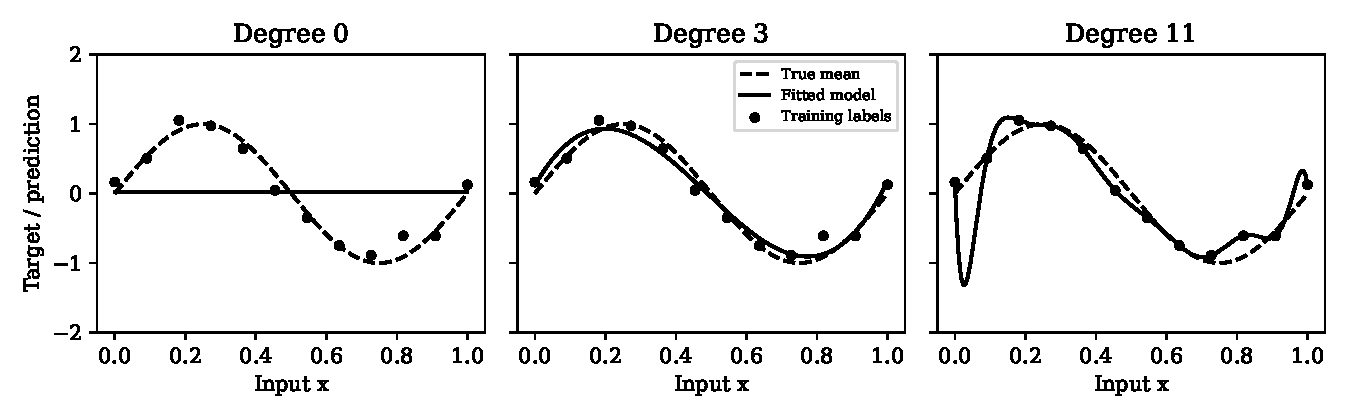
\includegraphics[width=.98\linewidth]{bias_variance/fits.pdf}
\caption{Constructed sine experiment: the same 12 noisy observations, with degrees 0, 3, and 11. Solid curves are fitted predictions; dashed curves are the conditional mean; dots are training labels. All panels share the plotted vertical range; extreme interpolating excursions may extend beyond it. Low training error alone does not certify accuracy between samples.}
\end{figure}

\subsection{Diagnosing generalization from results}
For $n_{\rm test}$ independent held-out examples, report
\[
\widehat R_{\rm test}=\frac1{n_{\rm test}}\sum_i(\hat f(x_i;\mathcal D)-y_i)^2,
\qquad \mathrm{RMSE}=\sqrt{\widehat R_{\rm test}}.
\]
MSE has squared target units; RMSE has target units. Compare like losses on comparable distributions. ``Low'' means low relative to a baseline, application tolerance, or attainable noise level, not a universal numeric threshold.
\begin{center}\small
\begin{tabular}{p{.24\linewidth}p{.32\linewidth}p{.33\linewidth}}
\toprule Pattern & Plausible diagnosis & Check before concluding\\\midrule
High training and test error & Underfitting / excessive restriction & Optimization failure, missing information, and high noise can also cause this.\\
Very low training error, much larger test error & Overfitting & Check leakage, sample size, and train--test distribution shift.\\
Low test error; modest gap & Useful generalization on this distribution & Check uncertainty, subgroup errors, and representative sampling.\\\bottomrule
\end{tabular}
\end{center}
The slide's ``perfect fit'' is a vivid example, not a necessary condition for overfitting. A model can overfit without zero training error. Similarly, underfitting is inadequate representation of the predictive structure, not merely failure to match every noisy label. A small train--test gap can coexist with very poor predictions. Plot residuals against $x$: systematic curvature suggests missing structure; large changes after resampling suggest instability. These are diagnostic clues, not isolated proofs.

\paragraph{Choosing $M$.} Fit coefficients on training data; compare candidate degrees on validation data or through cross-validation; evaluate the selected procedure once on an untouched test set. Repeatedly selecting degrees using test error turns that set into validation data. Even when only train and test results are supplied for diagnosis, this distinction matters for any subsequent model choice.

\paragraph{Predict before continuing (A2).} Three models have train/test MSE $(0.48,0.50)$, $(0.03,0.05)$, and $(0.0001,0.80)$ on comparable, sufficiently large splits. Which is the strongest candidate for each diagnosis? Can these numbers reveal the separate bias, variance, and noise components?

\section{Bias--variance tradeoff}
\subsection{Expectation means averaging over a specified source of variation}
\label{sec:reg:expect}
An expectation is a probability-weighted average, not necessarily the average of the particular observations in hand. For a discrete $Z$, $\E[Z]=\sum_z zp(z)$; with a density, $\E[Z]=\int z p(z)\,dz$. A conditional expectation uses a restricted population: $\E[Y\mid X=x]=\int y p(y\mid x)\,dy$ [S2]. For continuous $X$, this refers to a conditional distribution, rather than division by the probability of the zero-probability event $X=x$.

In the slide's seven-person table, the empirical height distribution assigns probabilities $2/7,4/7,1/7$ to $160,170,180$. Its mean is $1180/7\approx168.57$. Restricting to the three rows labelled $f$ changes the probabilities to $2/3,1/3,0$, and the conditional empirical mean becomes $490/3\approx163.33$. These are averages under the table's empirical distribution; population means need not equal them.

Linearity, $\E[aZ+bV]=a\E[Z]+b\E[V]$, follows by distributing a sum or integral and needs no independence. In contrast,
\[
\E[ZV]=\E[Z]\E[V]+\operatorname{Cov}(Z,V).
\]
Thus factorization holds for uncorrelated variables (with the necessary moments). Independence is sufficient but stronger. The universally valid conditional calculation is
\begin{equation}
\E[ZV]=\E_Z\!\left[Z\E[V\mid Z]\right].
\label{eq:reg:tower}
\end{equation}
At fixed $Z=z$, $z$ is a constant and can be pulled out; the outer expectation then averages over $Z$. This is the tower property applied to the product.

\begin{warning}[Clarification of slide S3]
The slide labels a factorization ``uncorrelated'' but its intermediate averaging notation can suggest that $\E[V\mid Z]=\E[V]$. Uncorrelatedness alone does not justify this intermediate substitution. The final factorization follows from zero covariance; independence (or mean independence in the required direction) justifies that substitution. We will explicitly condition whenever taking a factor outside an expectation.
\end{warning}
\paragraph{Optional counterexample.} Let $Z$ be uniform on $\{-1,0,1\}$ and $V=Z^2$. Symmetry gives $\E[ZV]=\E[Z^3]=0=\E[Z]\E[V]$, so they are uncorrelated. Yet $\E[V\mid Z]=Z^2$ varies with $Z$, and $V$ is completely determined by $Z$.

\subsection{Three functions, two experiments}
\label{sec:reg:random}
The notation in S4--S8 distinguishes three essential objects:
\begin{center}\small
\begin{tabular}{p{.19\linewidth}p{.39\linewidth}p{.31\linewidth}}
\toprule Symbol & Meaning & What is averaged?\\\midrule
$\bar y(x)$ & True conditional mean $\E[Y\mid X=x]$ & Fresh labels at the same input\\
$\hat f(x;\mathcal D)$ & Prediction after fitting one dataset & Nothing: one fitted predictor\\
$\bar f(x)$ & Mean fitted prediction $\E_{\mathcal D}[\hat f(x;\mathcal D)]$ & Repeated training datasets\\\bottomrule
\end{tabular}
\end{center}
The bar in $\bar y$ and $\bar f$ therefore represents different averaging operations. In the sine mechanism $\bar y(x)=\sin(2\pi x)$; it is not the observed noisy label. The function $\bar f$ is a theoretical average over repetitions, not generally a model we obtain from our one observed training set.

\paragraph{Experiment 1: freeze one trained model.} Once $\mathcal D$ is observed and fitting is deterministic, its learned weights are fixed. Draw a new independent pair $(X,Y)\sim\mathcal P$. Its loss is random because the pair is random. The risk of that fitted predictor is
\begin{equation}
R(\mathcal D)=\E_{X,Y}[(\hat f(X;\mathcal D)-Y)^2\mid\mathcal D]
=\iint(\hat f(x;\mathcal D)-y)^2p(x,y)\,dy\,dx.
\label{eq:reg:risk}
\end{equation}
Why the double integral? At every possible pair $(x,y)$ we calculate its squared loss, weight it by how likely that pair is, and sum continuously over both coordinates. It is the expectation definition applied to the \emph{function} $L(X,Y)$, not an expectation that updates the weights. Integrating over $y$ first averages possible labels at an input; integrating over $x$ averages how often each input appears.

\paragraph{Experiment 2: repeat the entire learning process.} Before collecting data, $\mathcal D\sim\mathcal P^N$ is random: each repetition provides $N$ fresh i.i.d. examples. A fixed degree and fixed fitting rule map each dataset to coefficients, so $\hat\theta(\mathcal D)$ and $\hat f(x;\mathcal D)$ become random across repetitions, even at a fixed query $x$. Now evaluate the \emph{procedure} by
\begin{equation}
\mathcal R=\E_{\mathcal D}[R(\mathcal D)]
=\iiint(\hat f(x;\mathcal D)-y)^2p(x,y)p(\mathcal D)\,d\mathcal D\,dy\,dx.
\end{equation}
The product density expresses independence of fresh test data and training data. For i.i.d. training samples, $p(\mathcal D)=\prod_{i=1}^N p(x_i,y_i)$; $d\mathcal D$ stands for integration over every training coordinate and label (or sums for discrete parts). We do not need to compute this enormous integral explicitly to reason about it. If the algorithm is randomized, include its random seed in the outer expectation too.

\paragraph{Why training MSE is only a proxy [S5].} For a predictor fixed independently of a sample, the sample mean of its losses estimates its population risk; with integrability, a law of large numbers explains convergence. But the fitted predictor is chosen using the training sample. Its training losses have been optimized, so this argument does not automatically establish that its training MSE is an unbiased estimate of its risk. A fresh test set restores independence for evaluation conditional on the fitted model. This is precisely the gap that overfitting exploits.

\paragraph{Reconstruction prompt (A3).} At a fixed $x$, list which of $Y$, $\bar y(x)$, $\hat f(x;\mathcal D)$, and $\bar f(x)$ vary when (i) only a new label is drawn, and (ii) only the training dataset is redrawn. Why is a single fitted model's error not itself its bias?

\subsection{Derive the decomposition at one input first}
\label{sec:reg:proof}
\paragraph{Assumptions.} We use squared loss and finite second moments, including $\E_{\mathcal D}[\hat f(x;\mathcal D)^2]<\infty$ at the inputs considered. A fresh test pair is independent of training data. Fix the training-set size and the learning rule. Let
\[
m=\bar y(x),\quad a=\bar f(x),\quad F=\hat f(x;\mathcal D),\quad
\sigma^2(x)=\Var(Y\mid X=x).
\]
For this derivation $x,m,a$ are fixed; $F$ varies over training sets and $Y$ varies over fresh conditional labels. This separation prevents most notation mistakes.

\paragraph{Step 1: separate variation between fitted models [S9--S10].}
Add and subtract the mean fitted prediction $a$:
\[
F-Y=(F-a)+(a-Y).
\]
Squaring and using linearity gives
\begin{align}
\E_{\mathcal D,Y\mid x}[(F-Y)^2]
&=\E_{\mathcal D}[(F-a)^2]+\E_{Y\mid x}[(a-Y)^2]\notag\\
&\quad+2\E_{Y\mid x}\!\left[(a-Y)\E_{\mathcal D}[F-a]\right].
\label{eq:reg:first}
\end{align}
For the cross term we first fix $x,y$, so $(a-y)$ is constant with respect to the dataset average. Test--training independence means this dataset average is the ordinary training-set average, unaffected by that fresh label. By the definition of $a$,
\[
\E_{\mathcal D}[F-a]=\E_{\mathcal D}[F]-a=a-a=0.
\]
Thus the cross term vanishes. Its \emph{individual realizations need not vanish}: positive and negative deviations cancel when averaged. The first remaining term is prediction variance $\Var_{\mathcal D}(F)$.

\paragraph{Pause (A4).} Explain why this reasoning can fail if $Y$ is one of the labels used to fit $F$. Identify the specific averaging step that changes; do not merely say ``overfitting.''

\paragraph{Step 2: separate mean-model error from unpredictable labels [S11].}
There is still variation inside $a-Y$. Insert the true conditional mean:
\[
a-Y=(a-m)+(m-Y).
\]
Now $a-m$ is constant under the label average, so
\begin{align}
\E_{Y\mid x}[(a-Y)^2]
&=(a-m)^2+\E_{Y\mid x}[(m-Y)^2]
 +2(a-m)\E_{Y\mid x}[m-Y]\notag\\
&=(a-m)^2+\sigma^2(x),
\end{align}
because $\E[Y\mid x]=m$. Notice that this second cancellation needs a zero \emph{conditional} mean, not merely $\E[m(X)-Y]=0$ globally.

\begin{keyidea}[Pointwise decomposition]
Define $b(x)=\bar f(x)-\bar y(x)$ and $v(x)=\E_{\mathcal D}[(\hat f(x;\mathcal D)-\bar f(x))^2]$. Then
\begin{equation}
\boxed{\E_{\mathcal D,Y\mid x}[(\hat f(x;\mathcal D)-Y)^2]
=b(x)^2+v(x)+\sigma^2(x).}
\label{eq:reg:decomp}
\end{equation}
Bias $b(x)$ is signed; the additive error contribution is \emph{bias squared}. All three terms on the right are nonnegative and have squared target units.
\end{keyidea}
Gaussian noise is unnecessary for this identity. Nor must noise variance be constant in $x$. Finite moments and the stated sampling conditions are what matter.

\paragraph{Step 3: average across inputs [S12].}
Use $p(x,y)=p(y\mid x)p(x)$ and the tower property:
\begin{equation}
\mathcal R=\E_X[b(X)^2]+\E_X[v(X)]+\E_X[\sigma^2(X)].
\label{eq:reg:integrated}
\end{equation}
The first term is the \emph{mean squared pointwise bias}, not $(\E_X[b(X)])^2$: opposite signed biases at different inputs must not cancel a prediction penalty. The lecture's extra $y$ subscript on the bias-squared expectation is harmless but unnecessary because its integrand no longer depends on $y$.

\paragraph{Why the conditional mean is the right target.}
For any fixed scalar prediction $c$ at $x$, the same second expansion yields
\[
\E[(c-Y)^2\mid x]=(c-\bar y(x))^2+\sigma^2(x).
\]
The second term cannot be changed by $c$; the first is minimized at $c=\bar y(x)$. Thus conditional-mean prediction is optimal under squared loss. ``Noise'' is irreducible \emph{given the available input information and distribution}; a new informative sensor feature may reduce it. It is not necessarily metaphysical randomness or measurement error alone.

\subsection{Interpret the components without confusing their experiments}
\label{sec:reg:interpret}
\textbf{Bias squared:} How far is the average predictor from the conditional mean? A consistently wrong shape across datasets suggests bias. \textbf{Variance:} How far do individual fitted predictions scatter around their own average at the same input? It is not variation of predictions across different inputs and not simply variance of the labels. \textbf{Noise:} How much do fresh labels vary around their conditional mean even if that mean were known?

\paragraph{Worked numerical example.} At one input the mean target is $2$, fresh-label variance is $0.25$, and three equally likely training outcomes predict $1,2,3$. Their average is $2$, so $b^2=0$ and $v=(1+0+1)/3=2/3$. Expected fresh-label squared error is $2/3+1/4=11/12$. For a direct check, let fresh labels be $1.5$ and $2.5$ with equal probabilities, independent of the model outcome. For predictions $1,2,3$, average squared losses are respectively $1.25,0.25,1.25$; averaging these gives $11/12$ again. Each fitted model may be imperfect even though the learning procedure has zero bias here.

\paragraph{Partially worked example (A5).} Shift the three predictions to $2,3,4$, retaining the same label distribution. Their mean is now $3$, hence $b=3-2=1$. Complete the variance and total-error calculations. Does translating all predictions change their spread?

\paragraph{Reading the lecture's pictures [S7, S13--S14].} In S7, each thin line is a model trained on a different dataset, while the highlighted mean line averages their predictions at each fixed $x$. A flat mean near zero can be stable yet miss the sine shape. In the darts analogy [S13], the bullseye corresponds to the true target, each dart to a retrained prediction, the dart cloud's centre to $\bar f$, and its spread to prediction variance. For scalar regression the darts would lie on a line; the two-dimensional board is only an analogy. It does not depict label noise unless an additional source of target variation is shown.

In S14, columns (a) and (b) show fixed functions repeated across $\mathcal D_1,\mathcal D_2,\mathcal D_3$: at a given input their dataset-induced variance is zero, even though their bias may be large and differs across inputs. Column (c) learns a cubic; column (d) learns an affine function. Both can vary across datasets. The illustration suggests flexibility versus stability, but three drawings cannot quantify population bias or variance, and do not prove a universal ordering.

\paragraph{Answering the lecture's consistent-error question.} A procedure that makes the same \emph{systematic prediction error relative to the conditional mean} across many training sets suggests high bias. The qualification matters: fresh noisy labels can cause unavoidable errors even for an unbiased predictor, and a single dataset cannot identify the components. Bias concerns a learning procedure and a target, not just the visible residual of one fitted model.

\subsection{A computational experiment that separates the sources}
\label{sec:reg:experiment}
\paragraph{Prediction and task (A6).} Before reading the reference code in the solutions: fit degrees $0,3,9$ to repeated noisy sine datasets. Predict which degree has the highest bias and which has the highest prediction variance. At a fixed input grid, store predictions in a matrix $P\in\R^{B\times G}$, where $B$ is the number of retrainings and $G$ the number of query inputs. Decide which axis to average. Explain why one model evaluated at many inputs is not a substitute for retraining.

The companion experiment fixes 12 training locations and redraws independent Gaussian label noise with $\sigma=0.15$ for 400 repetitions. This is a \emph{fixed-design variant} of the lecture's random-design experiment: the outer average is over noisy labels conditional on the chosen training inputs. It isolates one source of instability; it does not estimate the additional effect of random input locations. Evaluation averages over a uniform grid of 201 inputs, approximating a uniform input distribution. Degree 9 uses least squares, not interpolation of all 12 points.

At each grid point compute the replicate mean $\hat a$, mean squared deviation from $\hat a$, and squared deviation of $\hat a$ from the known sine mean. With divisor $B$ (not $B-1$), the finite-array identity
\[
\frac1B\sum_{r=1}^B(P_{rg}-m_g)^2
=(\hat a_g-m_g)^2+\frac1B\sum_{r=1}^B(P_{rg}-\hat a_g)^2
\]
is exact up to floating-point error. This verifies the algebra; the components are still Monte Carlo estimates of population quantities. Add the known $0.15^2$ noise variance to obtain conditional expected fresh-label MSE. A separate draw of independent test noise gives a noisy empirical check rather than an exact equality.
\begin{figure}[htbp]\centering
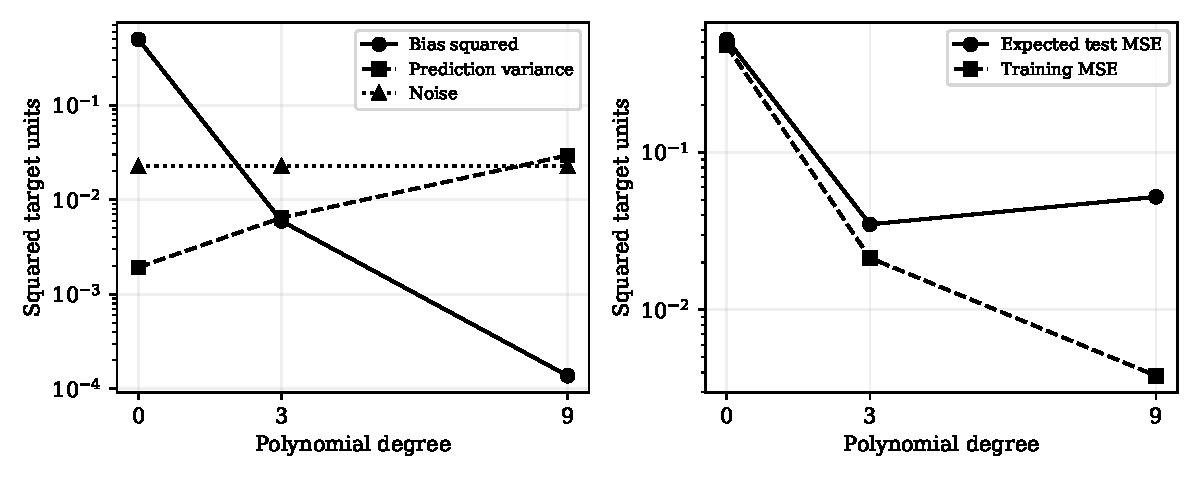
\includegraphics[width=.94\linewidth]{bias_variance/components.pdf}
\caption{Executed fixed-design experiment. Left: estimated integrated bias squared, prediction variance, and noise. Right: their sum compared with average training MSE. Logarithmic vertical scales separate the magnitudes; lines only connect the tested degrees. A lower training error need not mean a lower expected test error.}
\end{figure}
\begin{center}\small
\begin{tabular}{rrrrrr}
\toprule Degree & Training MSE & Bias$^2$ & Variance & Expected test & Noisy test\\
\midrule
0 & 0.47609 & 0.49753 & 0.00193 & 0.52195 & 0.52203\\
3 & 0.02136 & 0.00595 & 0.00645 & 0.03490 & 0.03489\\
9 & 0.00381 & 0.00014 & 0.02946 & 0.05209 & 0.05202\\
\bottomrule
\end{tabular}
\end{center}

The middle degree balances approximation and instability in this constructed setting. No rule says every test-error curve must be U-shaped. The exact decomposition survives cases where that familiar cartoon does not describe the behavior. Regularization will next provide another way to control the fitted procedure's sensitivity, beyond choosing the degree.

\subsection*{Compact reference sheet}
\begin{center}\small
\begin{tabular}{p{.40\linewidth}p{.49\linewidth}}
\toprule Quantity / equation & Meaning, conditions, use\\\midrule
$\hat R=N^{-1}\|\Phi\theta-\mathbf y\|^2$ & Observed training objective; $\Phi$ is $N\times(M+1)$. Fit coefficients, not certify generalization.\\
$R(\mathcal D)=\E_{X,Y}[(\hat f-Y)^2\mid\mathcal D]$ & Risk of one frozen fitted predictor on independent fresh data.\\
$\bar y(x)=\E[Y\mid x]$ & Squared-loss optimal target; requires a finite conditional second moment for this risk argument.\\
$\bar f(x)=\E_{\mathcal D}[\hat f(x;\mathcal D)]$ & Average over a specified retraining experiment, with fixed learning rule and sample size.\\
$b(x)=\bar f(x)-\bar y(x)$ & Signed systematic error of that procedure at one input.\\
$v(x)=\Var_{\mathcal D}(\hat f(x;\mathcal D))$ & Prediction sensitivity across training datasets at fixed $x$.\\
$\sigma^2(x)=\Var(Y\mid x)$ & Residual uncertainty given the input; can vary with $x$.\\
$\mathcal R=\E_X[b^2+v+\sigma^2]$ & Squared-loss decomposition; independent test data and finite moments.\\\bottomrule
\end{tabular}
\end{center}

\section*{Essential practice}
Complete these before consulting the hints. The short attempts A1--A6 in the text are also part of the practice sequence.
\begin{enumerate}[label=E\arabic*.,leftmargin=*]
\item \textbf{[O1, standard; nested models]} Prove that the optimal training MSE cannot increase from degree $M$ to $M+1$. Name two reasons an actual program might report an increase despite this theorem. State when $N$ arbitrary labels can be interpolated with degree at most $N-1$.
\item \textbf{[O3--O4, standard; reconstruct]} Close the derivation. Starting with $F-Y$, insert both $a=\E_{\mathcal D}F$ and $m=\E[Y\mid x]$, expand the resulting three-term square, and justify why each of the three cross terms vanishes. Specify what is fixed and which independence condition you use.
\item \textbf{[O5, standard; changed distribution]} At input $u$, bias is $-2$, prediction variance is $1$, and noise variance is $0.5$. At input $v$, these quantities are $1$, $4$, and $2$. Test inputs have probabilities $1/4$ and $3/4$. Compute total expected test MSE and each integrated component. Compare mean squared bias with squared mean bias.
\item \textbf{[O2--O3, standard; find the first invalid step]} A student writes: ``For every fixed $\theta$, training MSE is unbiased for risk. Therefore training MSE at the training-selected $\hat\theta$ is unbiased for $R(\hat\theta)$. I choose degree using the lowest test error over 100 trials and report that same test error.'' Identify both statistical problems. Propose an evaluation procedure.
\item \textbf{[O2--O5, integrative]} A simulated robot predicts a scalar grasp-position correction in centimetres from one sensor feature. At one safety-critical input the true mean is $2$ cm and conditional noise variance is $0.25$ cm$^2$. Three equally likely training outcomes produce predictions $(1.8,2.0,2.2)$ for procedure A and $(1.0,2.5,4.0)$ for B. Their training MSEs are $0.12$ and $0.01$ cm$^2$. Calculate expected fresh-label MSE for each procedure at this input, choose the better one under squared loss, and explain why training MSE gives a different ranking. Then suppose an independent test set has 90\% of inputs in an easy region and 10\% in a difficult region. A's conditional MSEs are $(0.10,1.00)$; B's are $(0.05,2.00)$. Choose by deployment-average MSE. Would that criterion alone suffice if errors in the difficult region have a strict safety tolerance? A satisfactory answer includes calculations, units, and a limitation of the decision criterion.
\item \textbf{[O3--O5, implementation]} Implement A6 without copying the reference code. Verify the finite-replicate identity pointwise, then compare against independently sampled noisy test labels. Increase test-noise repetitions and explain why discrepancies should typically shrink. Explain why changing the variance divisor to $B-1$ spoils the exact finite-array identity.
\end{enumerate}
\paragraph{Optional challenge [O4--O5].} Suppose the observation contains two features $X,Z$, but prediction initially uses only $X$. Use the conditional variance identity to explain why the average irreducible squared error cannot increase when $Z$ is also available. Does this guarantee that a finite-data fitted model using both features has lower test error?

\subsection*{Delayed review: attempt a few days later}
\begin{enumerate}[label=R\arabic*.]
\item The mean target is $-1$, noise variance is $0.4$, and equally likely retrained predictions are $-2,0$. Calculate expected test MSE without rereading the derivation.
\item A model always predicts zero, regardless of its training data. Which component must be zero? Which components can remain positive?
\item Explain to a colleague why $\E_X[b(X)^2]$ and $(\E_X[b(X)])^2$ answer different questions. Invent a two-input example.
\item You double the training-set size. Which term is determined solely by the data distribution and available features? Must the other two terms both decrease?
\end{enumerate}

\section*{Hints}
These are deliberately separated from the teaching text. Try the first hint before using the second.
\begin{description}[style=nextline]
\item[A1--A2] First: write down the new sample mean and compare the two losses separately. Next: symmetry keeps the affine slope simple; a small generalization gap can occur for a poor model.
\item[A3--A4] First: name the variable being redrawn. Next: if the test label helped train the predictor, averaging over datasets conditional on that label need not give $\bar f(x)$.
\item[A5--A6] First: deviations from a translated mean are unchanged. Next: predictions are rows indexed by retraining, so average along the row index while keeping each column's input fixed.
\item[E1] First: embed one coefficient vector in the larger space. Next: append a zero coefficient and compare feasible objective values.
\item[E2] First: use $(F-a)+(a-m)+(m-Y)$. Next: $\E_{\mathcal D}(F-a)=0$ and $\E_{Y\mid x}(m-Y)=0$; condition before factoring the remaining product.
\item[E3] First: square the signed biases before averaging. Next: use the stated input probabilities for every component.
\item[E4] First: ask whether the predictor is independent of the sample whose losses are averaged. Next: model selection itself uses information.
\item[E5] First: compute the mean and spread of each prediction triple. Next: the deployment mixture weights are not equal.
\item[E6] First: expand $P_{rg}-m_g=(P_{rg}-\hat a_g)+(\hat a_g-m_g)$. Next: deviations from their finite-sample mean sum to zero exactly.
\item[Optional challenge] Start with $\Var(Y\mid X)=\E[\Var(Y\mid X,Z)\mid X]+\Var(\E[Y\mid X,Z]\mid X)$.
\end{description}

\section*{Solutions and checks}
\subsection*{Prerequisite diagnostic}
\textbf{D1.} $(a+b)^2=a^2+2ab+b^2$. Zero mean alone is insufficient: if $B=A$ and $A$ takes $-1,1$ equally often, $\E[A]=0$ but $\E[AB]=1$. \textbf{D2.} $\E[Z]=2.5$, $\E[Z^2]=7$, hence $\Var(Z)=7-2.5^2=0.75$. \textbf{D3.} $\Phi$ is $10\times4$, $\theta$ is $4\times1$, predictions are $10\times1$. \textbf{D4.} Yes: new inputs and labels cause new losses even though the coefficients remain fixed.

\subsection*{Attempts embedded in the text}
\textbf{A1.} The new labels are $(1,1,2)$. The constant becomes $4/3$; the affine fit becomes $4/3+x/2$. The interpolating quadratic is $1+x/2+x^2/2$. At $x=0$, constant and affine predictions each move by $1/3$, whereas the quadratic moves by $1$. This measures sensitivity to this particular perturbation, not variance over a specified distribution of datasets.

\textbf{A2.} The first is a candidate for underfitting relative to the much better second model, the second for useful generalization, and the third for overfitting. Noise and split differences must still be checked. No pair of train/test MSEs uniquely identifies the three decomposition components. Repeated training and information about the conditional target are needed for a direct decomposition.

\textbf{A3.} With $x$ and the dataset fixed, fresh-label sampling changes only $Y$. With $x$ and a chosen label fixed, retraining changes only $\hat f(x;\mathcal D)$. Both bars are theoretical averages under fixed distributions and a specified procedure. The error of one fitted model contains a particular dataset deviation as well as any systematic bias and label noise.

\textbf{A4.} If $Y$ is a training label, $\E_{\mathcal D}[F-a\mid x,Y]$ need not be zero: knowing that label changes which fitted predictors are likely. One cannot replace it by the unconditional dataset mean $\E_{\mathcal D}[F-a]$. This is why the decomposition here evaluates fresh test error.

\textbf{A5.} Deviations from the new mean $3$ are still $-1,0,1$, so variance stays $2/3$. Bias squared becomes $1$, and expected squared error is $1+2/3+1/4=23/12$. Translation changes location but not spread.

\textbf{A6.} Average the $B$ rows to obtain one mean prediction for each of the $G$ inputs. The degree-0 fit is expected to miss the sine shape; the degree-9 fit is expected to be more noise-sensitive than degree 3. A single prediction curve's variation with $x$ mixes legitimate signal structure with errors; it cannot measure variation due to retraining at a fixed input. See the executed companion experiment for this setup's actual estimates.

\subsection*{Essential exercises}
\textbf{E1.} If $\theta$ is feasible at degree $M$, $(\theta^\top,0)^\top$ is feasible at degree $M+1$ and produces identical training predictions. Minimizing over a superset cannot increase the minimum. Finite precision, poor conditioning, or an incomplete optimizer can break the observed monotonicity. Changing the sample, objective, or constraints also invalidates the comparison. With distinct scalar inputs, the square degree-$(N-1)$ Vandermonde matrix is invertible and any labels have a unique interpolating polynomial of degree at most $N-1$. Repeated inputs with conflicting labels cannot be interpolated by a function.

\textbf{E2.} Write $A=F-a$, $B=a-m$, $C=m-Y$. Then $B$ is constant at $x$, $\E A=0$, $\E C=0$. Consequently $\E[AB]=B\E A=0$ and $\E[BC]=B\E C=0$. Independence of the training data and the fresh conditional label gives $\E[AC]=\E A\E C=0$ at this fixed input. The squares are $\E A^2=v(x)$, $B^2=b(x)^2$, $\E C^2=\sigma^2(x)$. This is the same result as the two-stage derivation, with all three cross terms exposed.

\textbf{E3.} At $u$ the error is $4+1+0.5=5.5$; at $v$ it is $1+4+2=7$. Weighted components are $1.75$ (bias squared), $3.25$ (variance), and $1.625$ (noise). Total $=6.625$, agreeing with $5.5/4+3(7)/4$. The mean signed bias is $(-2)/4+3/4=0.25$, whose square is $0.0625$, not $1.75$. Squaring after averaging conceals opposing errors.

\textbf{E4.} The first invalid step substitutes a data-dependent fitted parameter into a statement about a predictor fixed independently of that data. Optimizing on the same sample creates dependence and generally optimism. The second problem is selection on the alleged test set; its winning error is no longer an untouched final evaluation. Use training data for fitting, a validation set or cross-validation for choosing the whole procedure, and fresh held-out test data for final reporting. Preprocessing learned from data must also be fitted within the training portion of each split.

\textbf{E5.} A has mean $2$, zero bias, and variance $(0.04+0+0.04)/3=2/75\approx0.026667$ cm$^2$. Expected test MSE is $83/300\approx0.276667$ cm$^2$. B has mean $2.5$, squared bias $0.25$, and variance $(2.25+0+2.25)/3=1.5$ cm$^2$. Its expected test MSE is $2$ cm$^2$. Choose A at this input. B's lower training MSE does not compensate for its large retraining variability on fresh data. For the regional mixture, A has $0.9(0.10)+0.1(1.00)=0.19$ cm$^2$; B has $0.9(0.05)+0.1(2.00)=0.245$ cm$^2$. Choose A by average MSE. A safety requirement also needs region-specific and possibly tail-error criteria: even A may fail an unspecified tolerance. The exercise does not supply enough information to certify safety.

\textbf{E6.} The reference below implements the experiment and asserts its algebraic identity. Independent test noise creates random finite-sample cross terms; they average toward zero as independent repetitions increase, without guaranteeing monotonic improvement in every realized run. The $B-1$ divisor estimates a population variance with a correction, whereas the exact finite-array decomposition uses the empirical distribution assigning mass $1/B$ to each prediction. Mixing these definitions breaks the identity. Monte Carlo estimates of bias squared are also not automatically unbiased population estimates.

\paragraph{Reference implementation.} This script was executed for the figures and table. It uses only NumPy, Matplotlib, and Python's standard library. Run from the repository root with \texttt{python machine\_learning/code/bias\_variance.py}. Numerical assertions check the decomposition, direct enumeration of the worked example, and training-error monotonicity for nested least-squares models. The JSON output records the seed, experiment design, and realized errors.
\lstinputlisting[basicstyle=\ttfamily\scriptsize]{code/bias_variance.py}

\paragraph{Optional challenge solution.}
Averaging the conditional variance identity over $X$ gives
\[
\E[\Var(Y\mid X)]-\E[\Var(Y\mid X,Z)]
=\E[\Var(\E[Y\mid X,Z]\mid X)]\geq0.
\]
The Bayes noise floor cannot rise with more information. A finite-sample learner can still get worse through estimation variance, unsuitable modeling, or optimization; a lower attainable floor is not a guarantee that a particular method reaches it.

\subsection*{Delayed-review solutions}
\textbf{R1.} Mean prediction $-1$ gives zero bias; prediction variance is $1$, so total MSE $1.4$. \textbf{R2.} Dataset-induced prediction variance is zero. Bias squared and label noise can both be positive. \textbf{R3.} For two equally likely inputs with biases $-1,+1$, mean squared bias is $1$ while squared mean bias is $0$: opposite errors cancel only in the latter. \textbf{R4.} Conditional noise variance is unchanged if the distribution and features are unchanged. Bias and prediction variance can change; neither is universally guaranteed to decrease for every learning procedure.

\section*{Self-assessment}
For each objective, record \emph{followed}, \emph{completed with a hint}, \emph{justified independently}, or \emph{adapted to a changed problem}. Record the date and repeat a changed task later; reading once is not evidence of independent performance.
\begin{center}\small
\begin{tabular}{p{.12\linewidth}p{.78\linewidth}}
\toprule Objective & Observable evidence\\\midrule
O1 & Rebuild $\Phi$ and the normal equations; solve A1 and prove E1 without notes.\\
O2 & Diagnose A2, explain two alternative causes, and repair the evaluation in E4.\\
O3 & Explain A3 and A4 aloud, naming what is fixed in each expectation.\\
O4 & Derive E2 on a blank page, including every cross-term justification.\\
O5 & Solve E3 and E5, then implement E6 and explain its fixed-design limitation.\\\bottomrule
\end{tabular}
\end{center}

% Regularization methods will be added when the next lecture material is supplied.

% ============================================================
%  Chapter 4: Support Vector Machines
% ============================================================
\chapter{Support Vector Machines}
\label{ch:support_vector_machines}

% Sections not added yet. When you have them, create the folder
% chapters/04_support_vector_machines/ with one file per section and \input them here, e.g.
% \input{chapters/04_support_vector_machines/01_some_section}

% ============================================================
%  Chapter 5: Decision Trees
% ============================================================
\chapter{Decision Trees}
\label{ch:decision_trees}

% Sections not added yet. When you have them, create the folder
% chapters/05_decision_trees/ with one file per section and \input them here, e.g.
% \input{chapters/05_decision_trees/01_some_section}

% ============================================================
%  Chapter 6: Neural Networks (I)
% ============================================================
\chapter{Neural Networks (I)}
\label{ch:neural_networks_1}

% Sections not added yet. When you have them, create the folder
% chapters/06_neural_networks_1/ with one file per section and \input them here, e.g.
% \input{chapters/06_neural_networks_1/01_some_section}

% ============================================================
%  Chapter 7: Neural Networks (II)
% ============================================================
\chapter{Neural Networks (II)}
\label{ch:neural_networks_2}

% Sections not added yet. When you have them, create the folder
% chapters/07_neural_networks_2/ with one file per section and \input them here, e.g.
% \input{chapters/07_neural_networks_2/01_some_section}

% ============================================================
%  Chapter 8: Ensembles
% ============================================================
\chapter{Ensembles}
\label{ch:ensembles}

% Sections not added yet. When you have them, create the folder
% chapters/08_ensembles/ with one file per section and \input them here, e.g.
% \input{chapters/08_ensembles/01_some_section}

% ============================================================
%  Chapter 9: Gradient-Boosted Trees
% ============================================================
\chapter{Gradient-Boosted Trees}
\label{ch:gradient_boosted_trees}

% Sections not added yet. When you have them, create the folder
% chapters/09_gradient_boosted_trees/ with one file per section and \input them here, e.g.
% \input{chapters/09_gradient_boosted_trees/01_some_section}

% ============================================================
%  Chapter 10: Hyper-parameter Tuning
% ============================================================
\chapter{Hyper-parameter Tuning}
\label{ch:hyper_parameter_tuning}

% Sections not added yet. When you have them, create the folder
% chapters/10_hyper_parameter_tuning/ with one file per section and \input them here, e.g.
% \input{chapters/10_hyper_parameter_tuning/01_some_section}

% ============================================================
%  Chapter 11: Fighting Overfitting
% ============================================================
\chapter{Fighting Overfitting}
\label{ch:fighting_overfitting}

% Sections not added yet. When you have them, create the folder
% chapters/11_fighting_overfitting/ with one file per section and \input them here, e.g.
% \input{chapters/11_fighting_overfitting/01_some_section}

% ============================================================
%  Chapter 12: Error Metrics
% ============================================================
\chapter{Error Metrics}
\label{ch:error_metrics}

% Sections not added yet. When you have them, create the folder
% chapters/12_error_metrics/ with one file per section and \input them here, e.g.
% \input{chapters/12_error_metrics/01_some_section}


% ---------------- Bibliography ----------------
\bibliographystyle{plainnat}
% Course textbooks; remove once you cite things with \cite{...}
\nocite{bishop2006pattern, hastie2009elements, murphy2022probabilistic}
\bibliography{references}

\end{document}
